\section{Evaluation}
\label{sec:evaluation}

\vspace{-0.5em}
\subsection{Setups}
\label{sec:eval-setup}

\paragraph{Models.}
We evaluate \method{} on five hybrid linear-attention LLMs: Qwen3.5-9B, Qwen3.5-35B-A3B, and Qwen3.8-Flash use GDN~\citep{yang2025gated}; Kimi-Linear-48B-A3B-Instruct~\citep{team2025kimi} and GLM-5.3-Flash use KDA.
Due to limited hardware resources, we run only 8-layer versions of Qwen3.8-Flash and GLM-5.3-Flash on a single GPU, which preserve the per-layer decode cost but not the model output, and use them only for efficiency measurements.

\paragraph{Datasets and Evaluation.}
We use AIME 2026~\citep{maa2026aime}, GPQA-Diamond~\citep{rein2023gpqa}, MMLU-Pro~\citep{wang2024mmlu}, LiveCodeBench v6~\citep{jain2025livecodebench}, and GSM8K~\citep{cobbe2021gsm8k}.
We report downstream accuracy averaged over three random seeds.
For each model, all methods use the same prompts and the sampling parameters from its official model card (Appendix~\ref{app:eval-details}).
For decode and end-to-end efficiency, we compare against the FP32-state implementation of vLLM with CUDA graphs enabled.

\paragraph{Implementation.}
We implement \method{} in vLLM~\citep{kwon2023efficient} and write the linear attention decode kernels in TileLang~\citep{wang2025tilelang}. 
All other components (e.g., MoE layers) stay in the baseline precision.
At each window boundary, the compensator tokens are fitted with power iteration.
For all models and tasks, we use a window of $p=16$ tokens, $r=4$ FP16 Compensator Tokens ($r=8$ at 4 bits), and FP32 smoothing scales (Section~\ref{sec:ablation} studies $p$ and $r$).
All experiments run on NVIDIA B200, RTX PRO 6000, and RTX 5090 GPUs.

\paragraph{Baselines.}
We compare \method{} with the FP32 and BF16 states, the default and optional formats in vLLM and SGLang, and with state quantization baselines that re-quantize the state after every decode step.
At 8 bits, we evaluate FP8 and INT8 at their best granularities.
Given the lack of existing recurrent state quantization methods, we also evaluate three methods originally designed for the KV cache or activations, which we adapt to the recurrent state: KVQuant~\citep{hooper2024kvquant}, QuaRot~\citep{ashkboos2024quarot}, and TurboQuant~\citep{zandieh2026turboquant}.
At 6 and 4 bits, we evaluate NVFP6, MXFP6, and INT6, and NVFP4, MXFP4, and per-channel INT4, together with low-bit variants of the three adapted methods.
Table~\ref{tab:downstream} reports the best direct and adapted methods at each of these bit widths, and Appendix~\ref{app:full-results} lists all of them.

\subsection{Accuracy Results}
\label{sec:downstream}
\paragraph{Downstream tasks.}
Table~\ref{tab:downstream} shows the downstream accuracy of the three models.
With 8-bit quantization, \method{} achieves accuracy on par with the FP32 baseline across the 12 model--task pairs.
In contrast, per-step quantization leads to poor accuracy even at 16 bits: storing the Qwen3.5-9B state in BF16 lowers its AIME score from $87.9\%$ to $72.1\%$, whereas \method{} keeps $87.9\%$ with half as many bits.
This gap is especially clear on long generations: Qwen3.5-9B's AIME reasoning traces can run to tens of thousands of tokens, and per-step FP8 achieves only 14.6\% on AIME, versus 87.9\% for FP32.
Kimi-Linear-48B-A3B-Instruct produces shorter outputs and is less sensitive to per-step 8-bit storage; on AIME, GPQA, and LiveCodeBench, BF16, KVQuant, and QuaRot remain within 5\% of FP32.

\paragraph{Lower bit widths.}
The gap between per-window and per-step quantization widens as the bit width decreases.
At 6 bits, the best baselines, NVFP6 and TurboQuant, average only 29.6\% and 31.9\%, and both collapse on the Qwen models, while \method{} averages 72.4\%, close to FP32's 75.5\%.
At 4 bits, MXFP4 and TurboQuant average 9.7\% and 22.9\% and collapse on the Qwen models, while \method{} still averages 60.4\% and stays within 1.1\% of FP32 on every task of Kimi-Linear-48B-A3B.
These results show that \method{} retains substantially more downstream accuracy than the baselines even under aggressive 4-bit state quantization.

\subsection{Efficiency Results}
\label{sec:efficiency}

\begin{figure}[t]
    \centering
    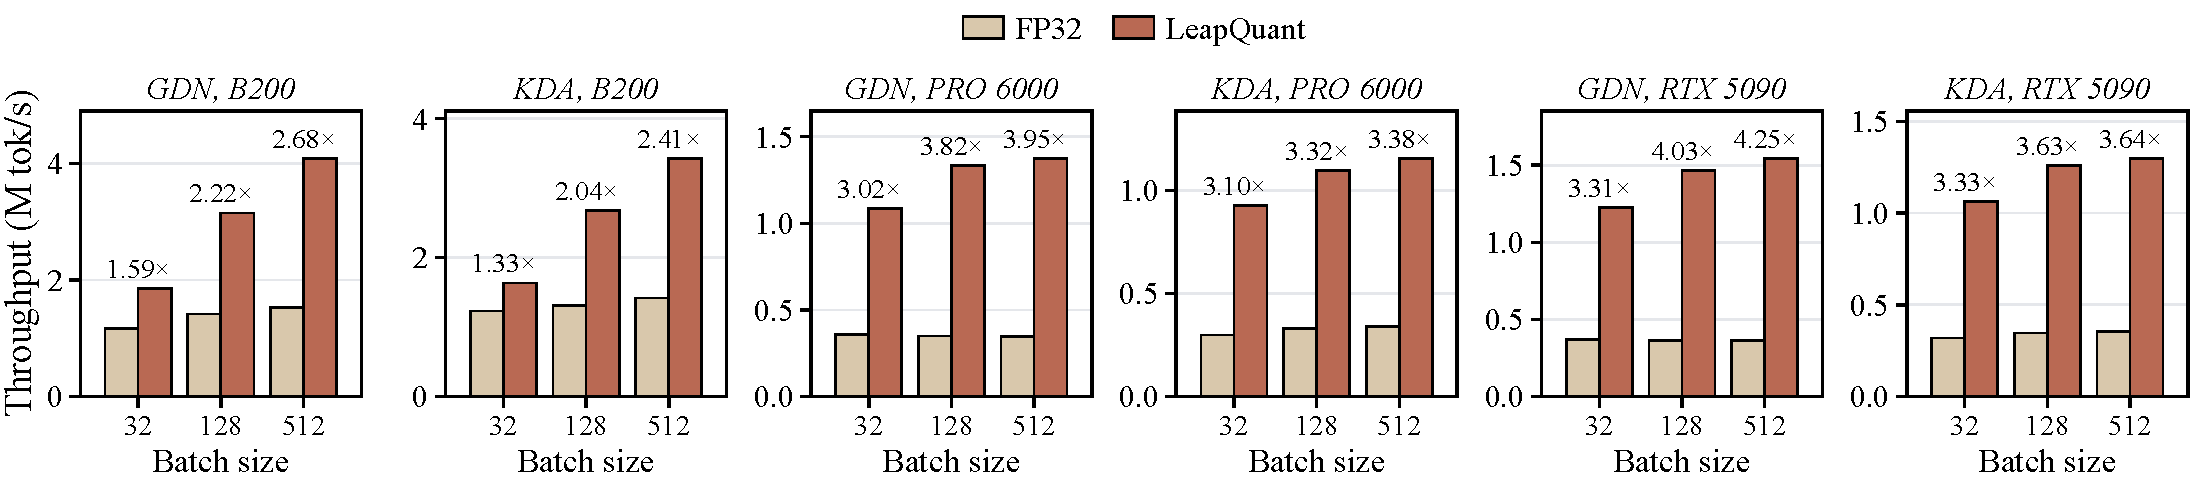
\includegraphics[width=\linewidth]{figures/eval_kernel.pdf}
    \caption{Kernel throughput of one linear attention layer.}
    \label{fig:eval-kernel}
\end{figure}

\begin{figure}[t]
    \centering
    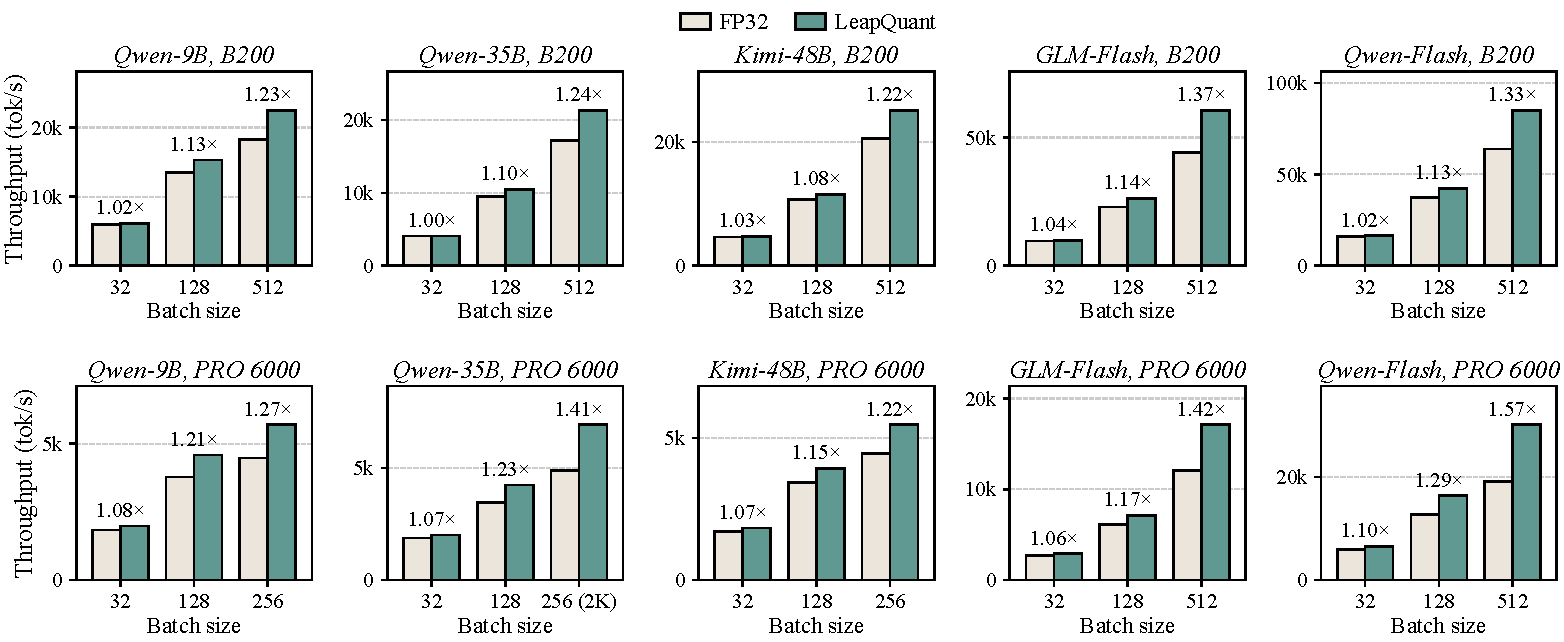
\includegraphics[width=\linewidth]{figures/eval_decode.pdf}
    \caption{Decode-step throughput in vLLM at context length 4K. On the RTX PRO 6000, the largest batch size is 256 where 512 does not fit, and Qwen3.5-35B-A3B uses 2K instead of 4K at this batch size.}
    \label{fig:eval-e2e}
\end{figure}


\paragraph{Kernel speedup.}
Figure~\ref{fig:eval-kernel} compares one linear attention layer (32 heads, $d_k=d_v=128$) with the FP32 kernel in FLA.
At batch size 512, \method{} is 2.68$\times$, 3.95$\times$, and 4.25$\times$ faster on GDN and 2.41$\times$, 3.38$\times$, and 3.64$\times$ on KDA on the B200, RTX PRO 6000, and RTX 5090.
The larger gains on the RTX PRO 6000 and RTX 5090 are consistent with recurrent-state traffic being a stronger bottleneck on these GPUs.

\paragraph{Decode speedup.}
Figure~\ref{fig:eval-e2e} measures pure decode steps on five hybrid models at context length 4K.
At batch size 512 on the B200, \method{} improves decode throughput by 1.22--1.37$\times$; at the largest batch size that fits on the RTX PRO 6000, the gain is 1.22--1.57$\times$. The gain increases with batch size as linear attention takes a larger share of each step.
Appendix~\ref{app:efficiency} reports other context lengths, up to 128K.

\begin{figure}[t]
    \centering
    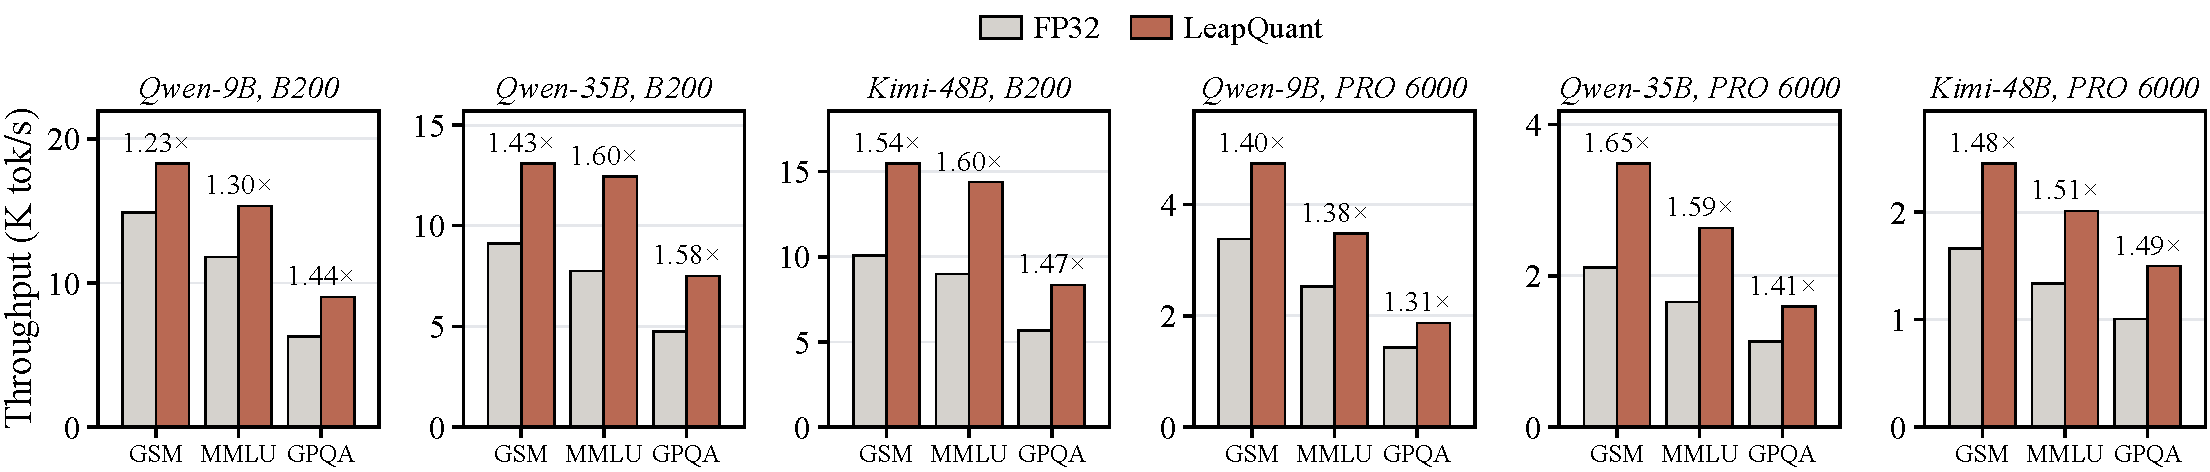
\includegraphics[width=\linewidth]{figures/eval_prefix.pdf}
    \caption{End-to-end inference throughput on different datasets.}
    \vspace{-1em}
    \label{fig:prefix}
\end{figure}


\paragraph{Memory reduction.}
\method{} stores each window-boundary state at 1.19 bytes per element instead of 4, including the INT8 residual, the smoothing scales, and the Compensator Tokens, a 3.4$\times$ reduction.
At a window length of 16, the FP16 update buffer requires only around 8 KiB per head per layer for 128$\times$128 states and is allocated once per active request, making its overhead marginal.
When prefix caching is enabled in the default mode in vLLM and SGLang, a checkpoint is kept per 1K cached tokens.
In this setting, \method{} reduces the end-to-end memory by 41\%, 51\%, and 56\% on Qwen3.5-9B, Qwen3.5-35B-A3B, and Kimi-Linear-48B-A3B.
This allows up to 1.4$\times$ more concurrent requests when serving the Qwen3.5-9B model on one B200 GPU.

\paragraph{End-to-end inference speedup.}
We run offline inference on GSM8K, MMLU-Pro, and GPQA with the input and output lengths of the original model.
Since Kimi-Linear is a non-reasoning model, we use the distribution of Qwen3.5-9B for it to simulate the real workload of production KDA models.
With more concurrent requests and faster decode steps, \method{} improves the output throughput by 1.23--1.60$\times$ on the B200 and 1.31--1.65$\times$ on the RTX PRO 6000 (Figure~\ref{fig:prefix}).

\vspace{-0.5em}
\subsection{Ablation Study}
\label{sec:ablation}

We ablate the design choices of \method{} on Qwen3.5-9B, using AIME 2026 and LiveCodeBench v6 as the most sensitive tasks in Table~\ref{tab:downstream}; kernel speedups are over the FP32 kernel at batch size 256.

\begin{wraptable}[12]{r}{0.43\linewidth}
  \vspace{-13pt}
  \raggedright
  \caption{\protect\raggedright Ablation of individual \method{} components on Qwen3.5-9B.}
  \label{tab:ablation}
  \centering
  \small
  \setlength{\tabcolsep}{0.5pt}
  \begin{tabular*}{\linewidth}{@{\extracolsep{\fill}}lccc@{}}
    \toprule
    Method & AIME & LCB & Kernel\\
    \midrule
    FP32 per-step & \textbf{87.9} & \textbf{64.1} & 1.00$\times$\\
    \midrule
    BF16 per-step & 72.1 & 49.6 & 1.64$\times$\\
    + Per-window & \textbf{87.8} & 62.9 & 1.71$\times$\\
    \midrule
    INT8 per-step & 7.1 & 9.2 & 2.43$\times$\\
    + Per-window & 82.4 & 60.6 & 2.64$\times$\\
    + Comp.\ Tokens & 86.6 & 61.5 & 2.56$\times$\\
    + Smoothing & \textbf{87.9} & \textbf{64.1} & 2.52$\times$\\
    \bottomrule
  \end{tabular*}
  \vspace{-8pt}
\end{wraptable}
\paragraph{Effectiveness of each design.}
Table~\ref{tab:ablation} adds the designs one at a time to an INT8 state, with BF16 as a higher-precision reference.
Per-step INT8 drops AIME from 87.9\% to 7.1\% and LiveCodeBench from 64.1\% to 9.2\%.
Per-window quantization improves AIME and LiveCodeBench accuracy to 82.4\% and 60.6\%, respectively; with BF16, it also raises AIME from 72.1\% to 87.8\%.
Compensator Tokens then improve the INT8 scores to 86.6\% and 61.5\%, while smoothing closes the remaining gap to FP32 at 2.52$\times$ kernel speedup.
Each stage improves quality while the complete 8-bit method retains a substantial efficiency advantage.
For efficiency, we compare against the FP32 and BF16 per-step FLA kernels and the BF16 ReplaySSM kernel in the official repository~\citep{dao2026replayssm}.
With all three components, \method{} matches FP32 accuracy at a 2.52$\times$ kernel speedup.

\begin{wraptable}{r}{0.48\linewidth}
  \vspace{-14pt}
  \raggedright
  \caption{\protect\raggedright Ablations of window length $p$ and Compensator Token count $r$ on Qwen3.5-9B.}
  \label{tab:ablation-pr}
  \centering
  \begin{minipage}[t]{0.48\linewidth}
    \centering
    \small
    \setlength{\tabcolsep}{0.5pt}
    \begin{tabular*}{\linewidth}{@{\extracolsep{\fill}}cccc@{}}
      \toprule
      $p$ & AIME & LCB & Kernel \\
      \midrule
      4 & 86.2 & 62.8 & 1.59$\times$ \\
      8 & 87.1 & 63.2 & 2.13$\times$ \\
      16 & \textbf{87.9} & \textbf{64.1} & \textbf{2.52$\times$} \\
      32 & \textbf{87.9} & \textbf{64.2} & 2.20$\times$ \\
      \bottomrule
    \end{tabular*}
  \end{minipage}\hfill%
  \begin{minipage}[t]{0.48\linewidth}
    \centering
    \small
    \setlength{\tabcolsep}{0.5pt}
    \begin{tabular*}{\linewidth}{@{\extracolsep{\fill}}cccc@{}}
      \toprule
      $r$ & AIME & LCB & Kernel \\
      \midrule
      2 & 85.7 & 63.4 & \textbf{2.57$\times$} \\
      4 & 87.9 & \textbf{64.1} & 2.52$\times$ \\
      8 & \textbf{88.1} & \textbf{64.0} & 2.37$\times$ \\
      16 & 87.9 & 62.8 & 0.74$\times$ \\
      \bottomrule
    \end{tabular*}
  \end{minipage}
  \vspace{-8pt}
\end{wraptable}
\paragraph{Window length.}
Table~\ref{tab:ablation-pr} (left) varies the window size $p$ with $r=4$.
Longer windows quantize less often, so accuracy improves up to $p=16$ and then saturates.
The kernel is fastest at $p=16$: shorter windows reconstruct the state more often, while longer ones enlarge the record buffer read at every step and leave less shared memory for pipelining.
$p=32$ gives no further accuracy gain, but its kernel speedup drops from 2.52$\times$ to 2.20$\times$ due to the increased memory traffic.

\noindent\begin{minipage}{\linewidth}
\paragraph{Number of Compensator Tokens.}
Table~\ref{tab:ablation-pr} (right) varies $r$ with $p=16$.
Accuracy saturates at $r=4$, consistent with the energy concentrated in a few singular values (Figure~\ref{fig:energy}).
Efficiency-wise, the power iteration and reconstruction work of up to four compensator tokens is fully overlapped with the memory reads on the B200 GPU, but it becomes exposed for larger $r$ and makes the kernel even slower than FP32 at $r=16$.
We therefore use $r=4$, which matches the accuracy of larger $r$ at nearly the kernel speed of $r=2$.
\end{minipage}
